\documentclass{article}

\usepackage[toc]{appendix}
\usepackage[english]{babel}
\usepackage[a4paper,top=2cm,bottom=2cm,left=3cm,right=3cm,marginparwidth=1.75cm]{geometry}
\usepackage{amsmath,amssymb}
\usepackage{graphicx}
\usepackage{xcolor}
\usepackage[colorlinks=true, allcolors=blue]{hyperref}
\usepackage{float} %for å kontrollere bildeplasseringene 
\usepackage{caption}
\usepackage{lipsum}
\usepackage[skip=0pt]{caption}


\renewcommand\thesubsection{\alph{subsection})} %Gjør at subsection blir a) i stedet for 1.1.1
\newcommand{\vect}[1]{\boldsymbol{{#1}}} %en ny kommando som sier at \vect gir fet skrift. det er alternativ vektornotasjon.


\title{Oppgave 1 - Geometri som beveger seg i fluid}
\author{Ole Sandok}

\begin{document}
\maketitle

\tableofcontents

\section{Randverdi i 2 dimensjoner}
Vi har en geometri som beveger seg med en fart U i et ubegrenset fluid. Bevegelsen i fjernfeltet er null. 

Løsningen på problemet finnes ved å løse integrallikningen:
\begin{equation}
    -\pi \phi(\bar{x}\bar{y})  + \int_{S} \phi  \frac{\partial }{\partial n} \ln r dS = \int_{S}  \frac{\partial \phi}{\partial n} \ln r dS
\end{equation}
der $\partial \phi / \partial n = n_1$ langs med S.

Integrallikning på diskret form.
\begin{equation}
    -\pi \phi  + \Sigma_{m=1}^N \phi_m (-\Delta \Theta_{n,m})   =  \sum_{m=1}^N [\frac{\partial \phi}{\partial n}]_m h_{n,m}
\end{equation}

Addert masse kan approksimeres slik:
\begin{equation}
    m_{ij}  = \rho \int_{S} \phi_j n_i dS \, \simeq \, \rho \sum_{m=1}^N [\phi_j]_m  [n_i]_m \Delta S_m.
\end{equation}


\section{Sirkel - Plott av addert masse og plott av potensialer}

{\noindent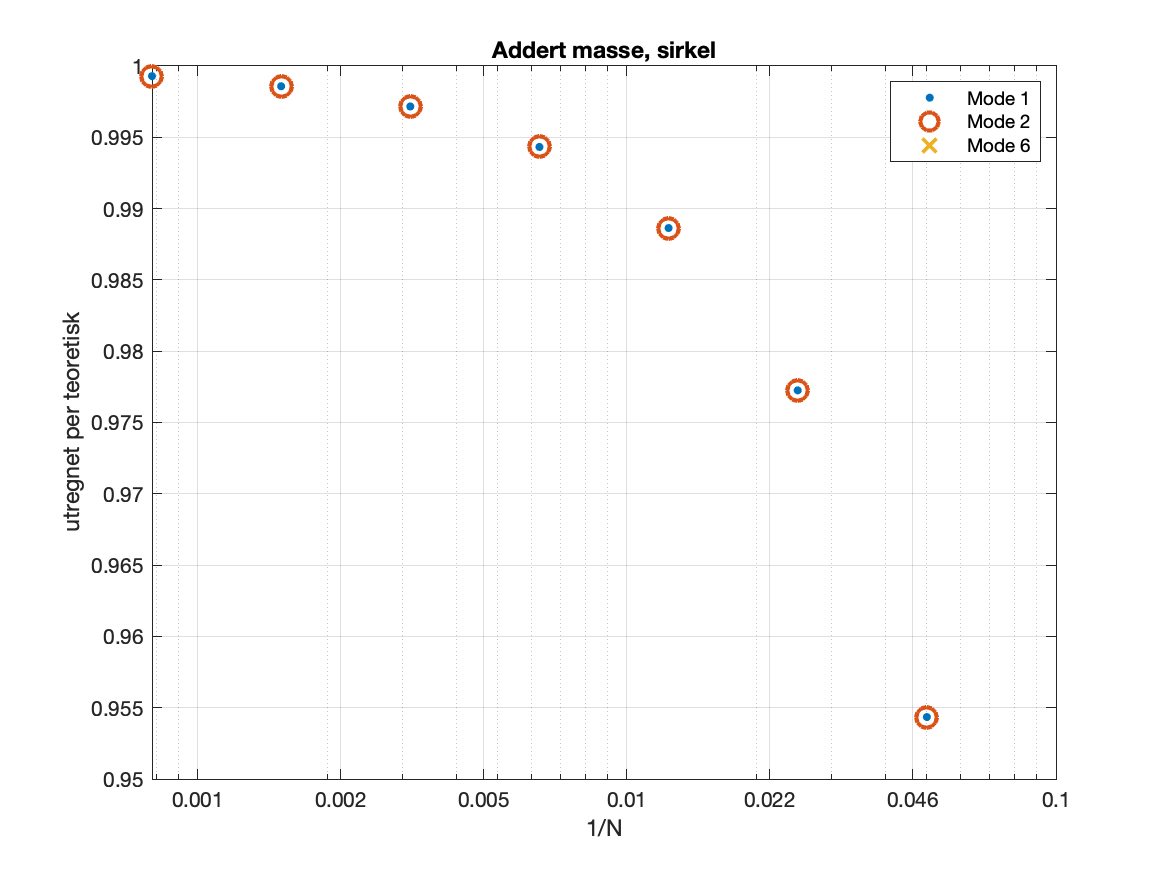
\includegraphics[width=0.8\linewidth]{/Users/ole/Tex/MEK4420/oblig1images/m11_sirkel.png}
\captionof{figure}{Plott der vi sammenlikner den utregnede med teoretiske adderte massen. Vi ser et tydelig samsvar mellom teori og diskret utregning. En økning i N antall diskrete punkter viser at simulerte modellen nærmer seg den teoretiske. Sirkelen er symmetrisk, så horisontal og vertikal bevegelse gir nøyaktig samme adderte masse. Allerede ved første diskretisering, N=20, så har vi over 95\% samsvar mellom teoretisk og utregnet. Som vi vil se i de neste plottene, varierer dette veldig mellom geometriene.}}

{\noindent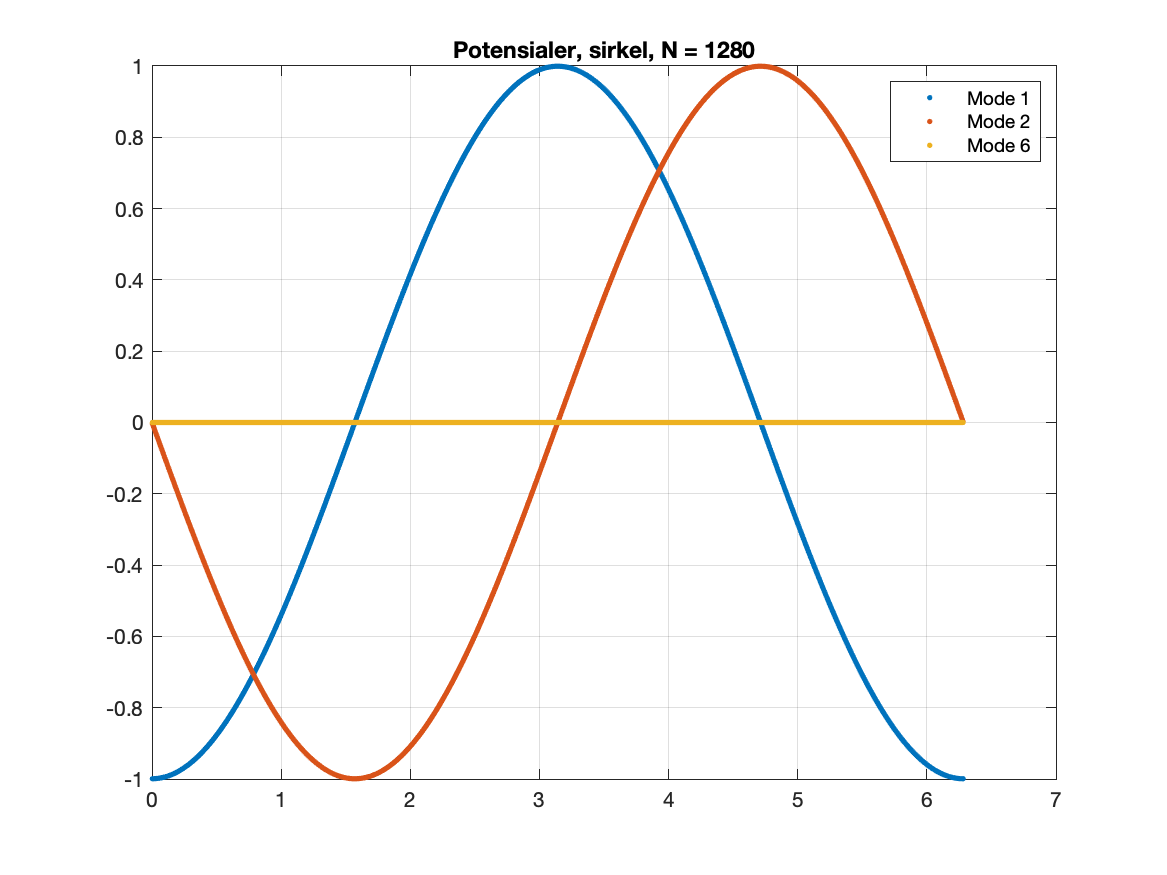
\includegraphics[width=0.8\linewidth]{/Users/ole/Tex/MEK4420/oblig1images/potensialer_sirkel.png}
\captionof{figure}{Vi ser at potensialene er identiske i fasong fra 0 til 2 pi, der mode 1 viser en minus cosinus-kurve, mode 2 en minus sinus kurve. Dvs at når sirkelen beveger seg horisontalt, mode 1, så er potensialet størst i bakkant, der sirkelen er =pi, og minst i front, eller høyre side =0=2pi. Denne sirkelen beveger seg altså til høyre. Rotasjon, mode 6 har intet potensial, ingen masse flyttes på når den glatte sirkelen roterer, så vi ser det stemmer at mode 6 er lik null.}}



%--------------------ellipse b/a = 0.1
\section{Ellipse - Plott av addert masse og plott av potensialer}

{\noindent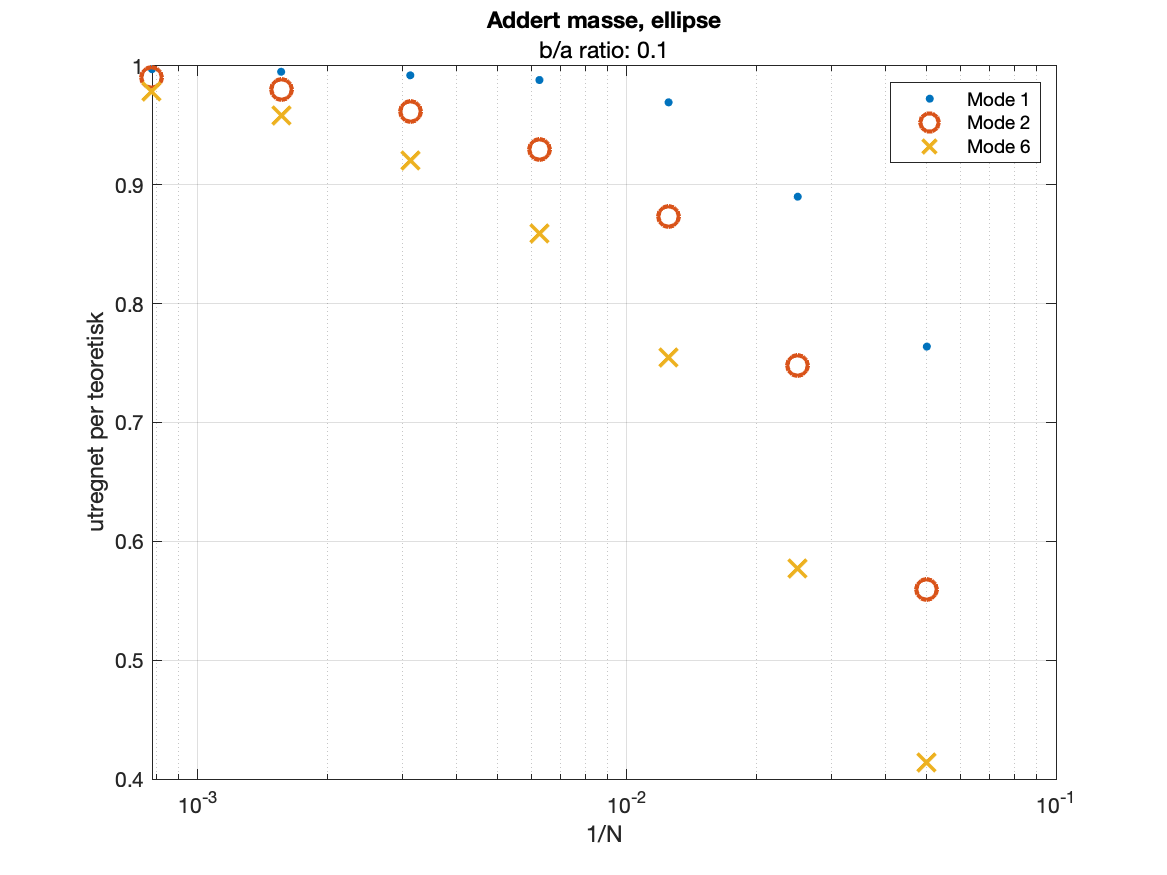
\includegraphics[width=0.8\linewidth]{/Users/ole/Tex/MEK4420/oblig1images/m11_ellipse.png}
\captionof{figure}{Vi sammenlikner utregnet og teoretisk addert masse for en bred ellipse. Bredden er 10x høyden. Vi ser at den horisontale bevegelsen, mode 1, trenger få punkter for at diskretiseringen skal samsvare godt med den teoretiske verdien. Vertikal bevegelse krever dobbelt så mange diskretiseringspunkter for tilsvarende samsvar. Rotasjon, mode 6, krever så omtrent dobbelt antall N som den vertikale, for tilsvarende samsvar. Verdier for N = 20,40,80,160,320,640,1280. }}

{\noindent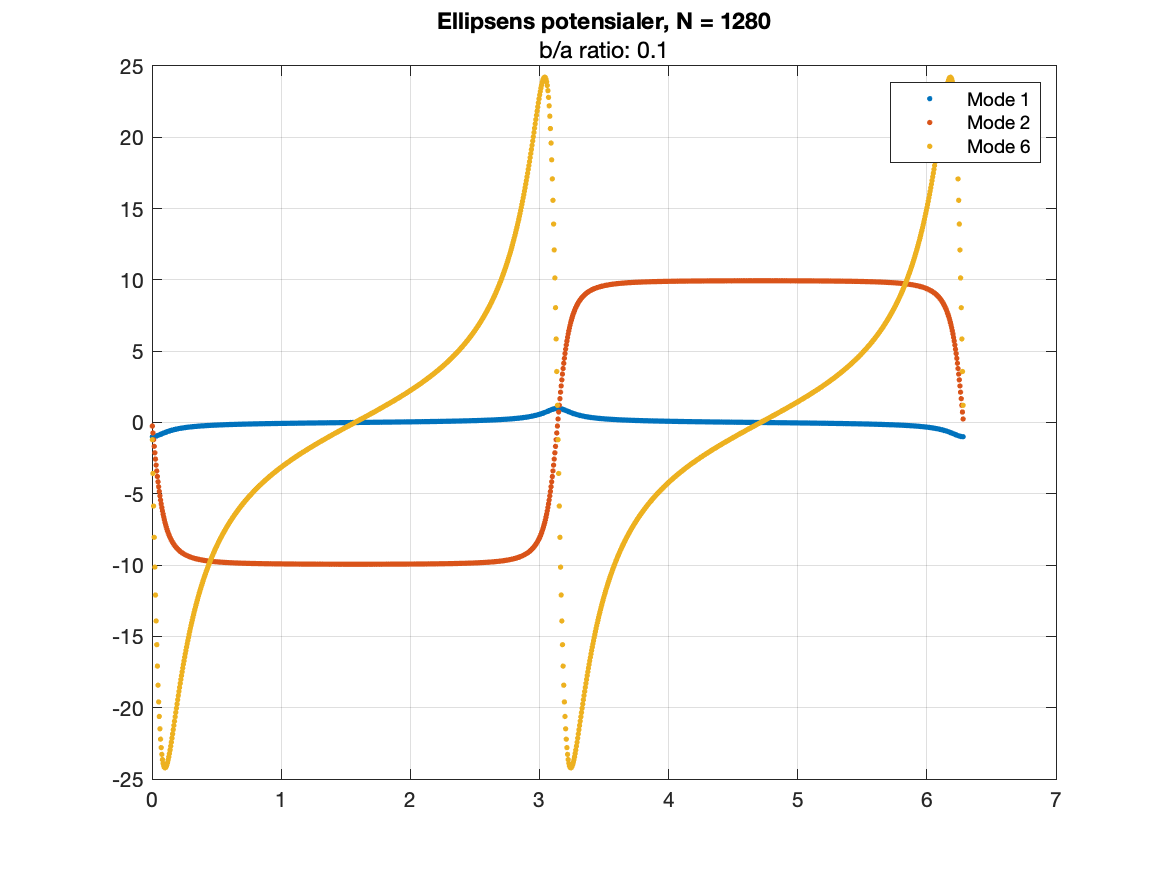
\includegraphics[width=0.8\linewidth]{/Users/ole/Tex/MEK4420/oblig1images/potensialer_ellipse.png}
\captionof{figure}{Ellipsens potensialer er svært ulike. Mode 1 har -1 i front og 1 i bakkant av ellipsen. Mode 2 har 10 ganger så mye, langs med toppen og bunnen. Rotasjonen, mode 6, viser svært stor respons på sidene av ellipsen. Som gir mening, det er ytterst på vår brede ellipse at mest vann fortrenges.}}


%--------------------ellipse b/a = 0.5
\subsection{En "ganske rund" ellipse}
{\noindent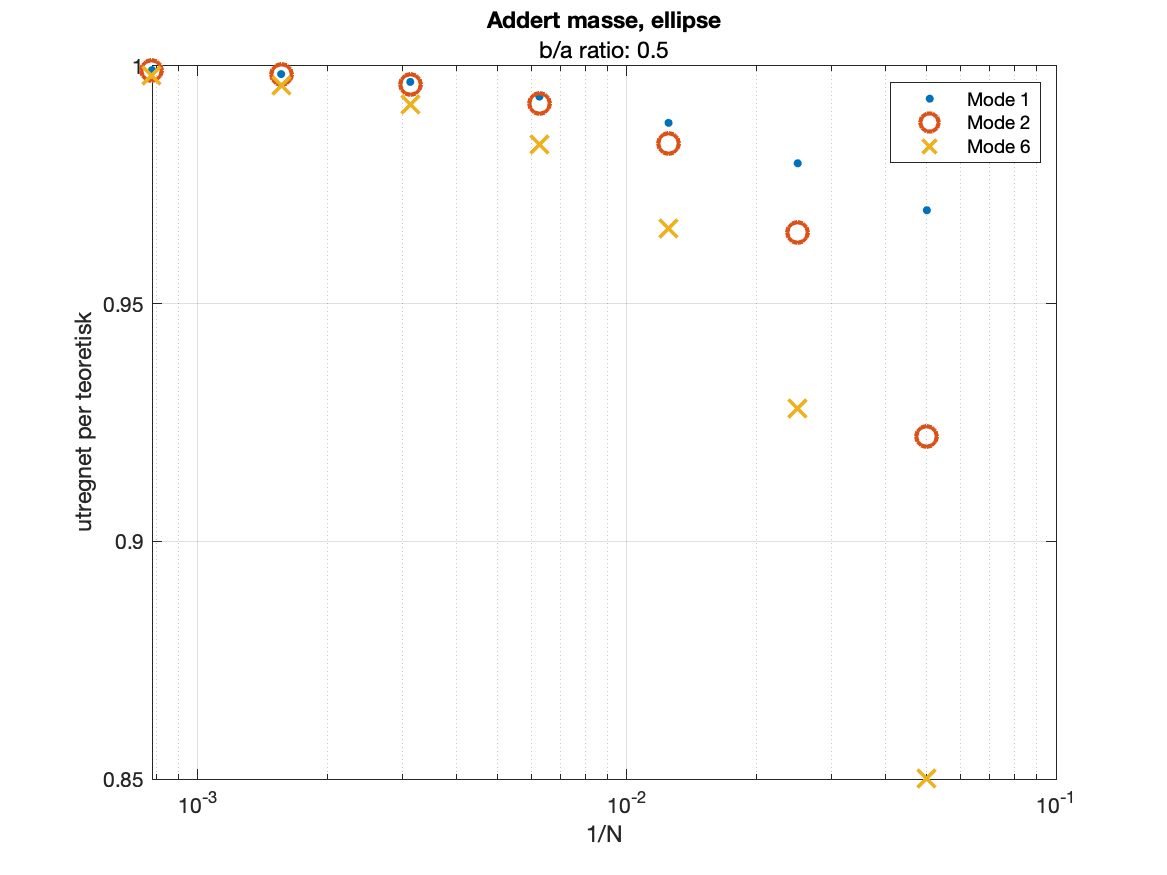
\includegraphics[width=0.8\linewidth]{/Users/ole/Tex/MEK4420/oblig1images/m11_2ellipse.png}
\captionof{figure}{Denne mer sirkulære ellipsen trenger mye færre punkter for å oppnå samme samsvar mellom teoretisk og utregnet addert masse. Over 95\% samsvar etter bare 20, 40 og 80 punkter for henholdsvis mode 1, 2 og 6.}}

{\noindent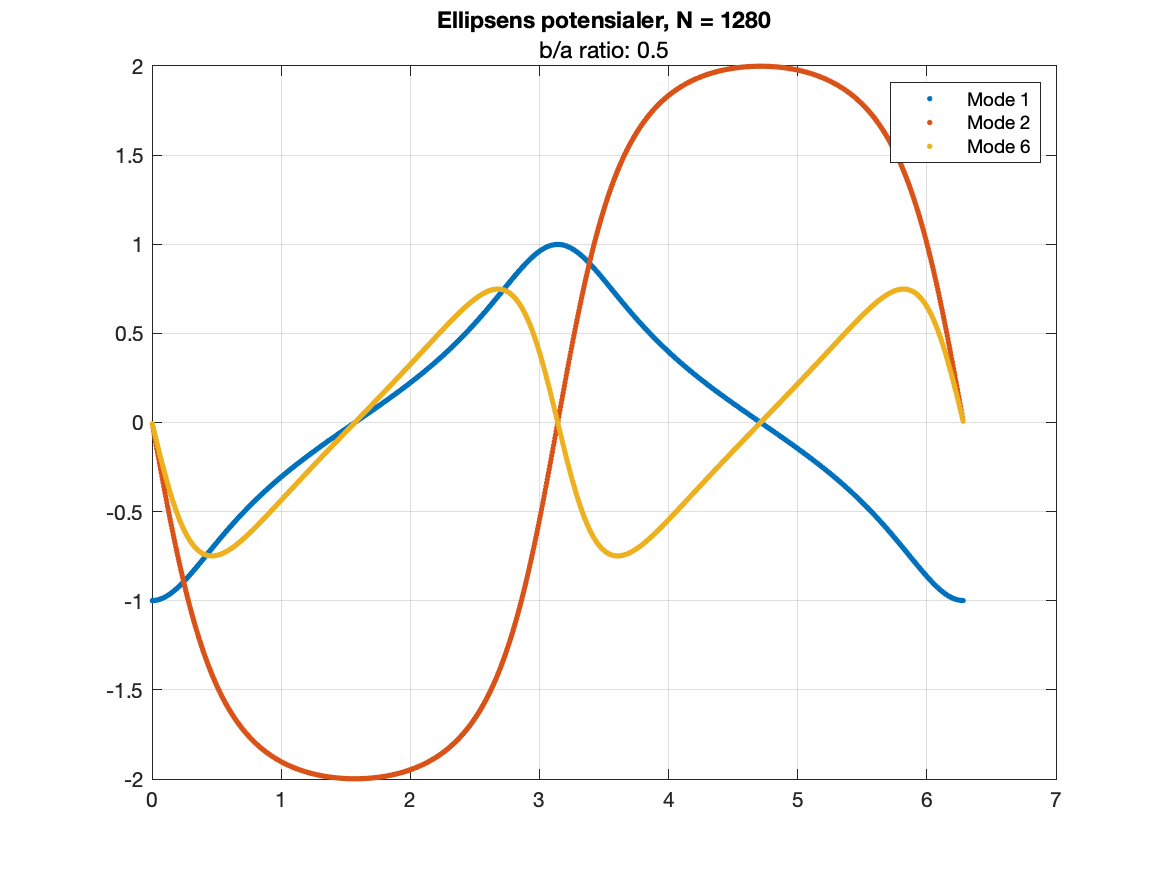
\includegraphics[width=0.8\linewidth]{/Users/ole/Tex/MEK4420/oblig1images/potensialer_2ellipse.png}
\captionof{figure}{For denne mer sirkulære ellipsen ser vi at den vertikale bevegelsen gir større forskjell i potensial enn rotasjonen.}}


%--------------------diskretisering ellipse
\subsection{Diskretisering av ellipse}
Vi tar en kjapp titt på diskretiseringen av ellipsen. Tilsynelatende bør vi bruke den jevne fordelingen, en vanlig ellipse merket med blå sirkler. Men den mer kompliserte inndelingen, merket med røde kryss, ble valgt fordi der endrer Arcustangens seg med en konstant verdi. 
{\noindent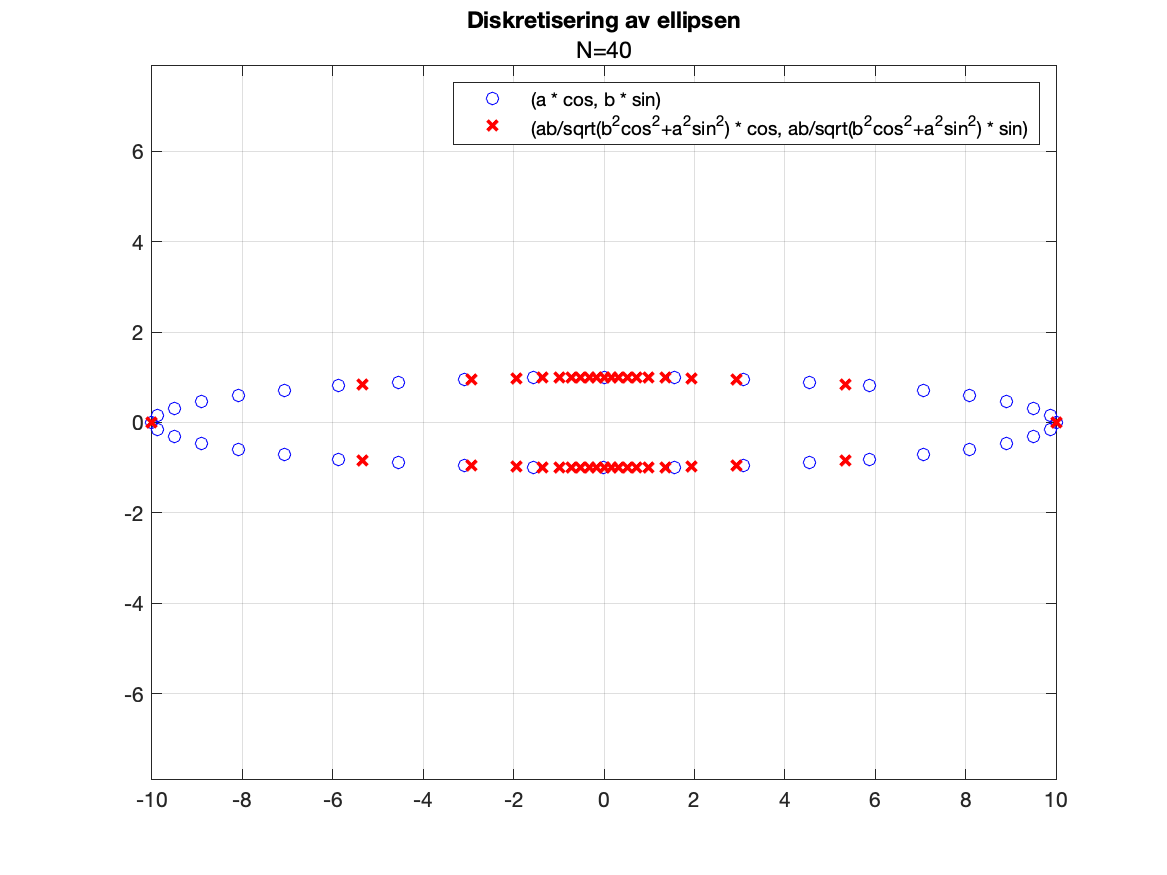
\includegraphics[width=0.8\linewidth]{/Users/ole/Tex/MEK4420/oblig1images/diskretisering_ellipse.png}
\captionof{figure}{de røde kryssene er fordelingen som er brukt. De blå sirklene er "normal" fordeling}}

{\noindent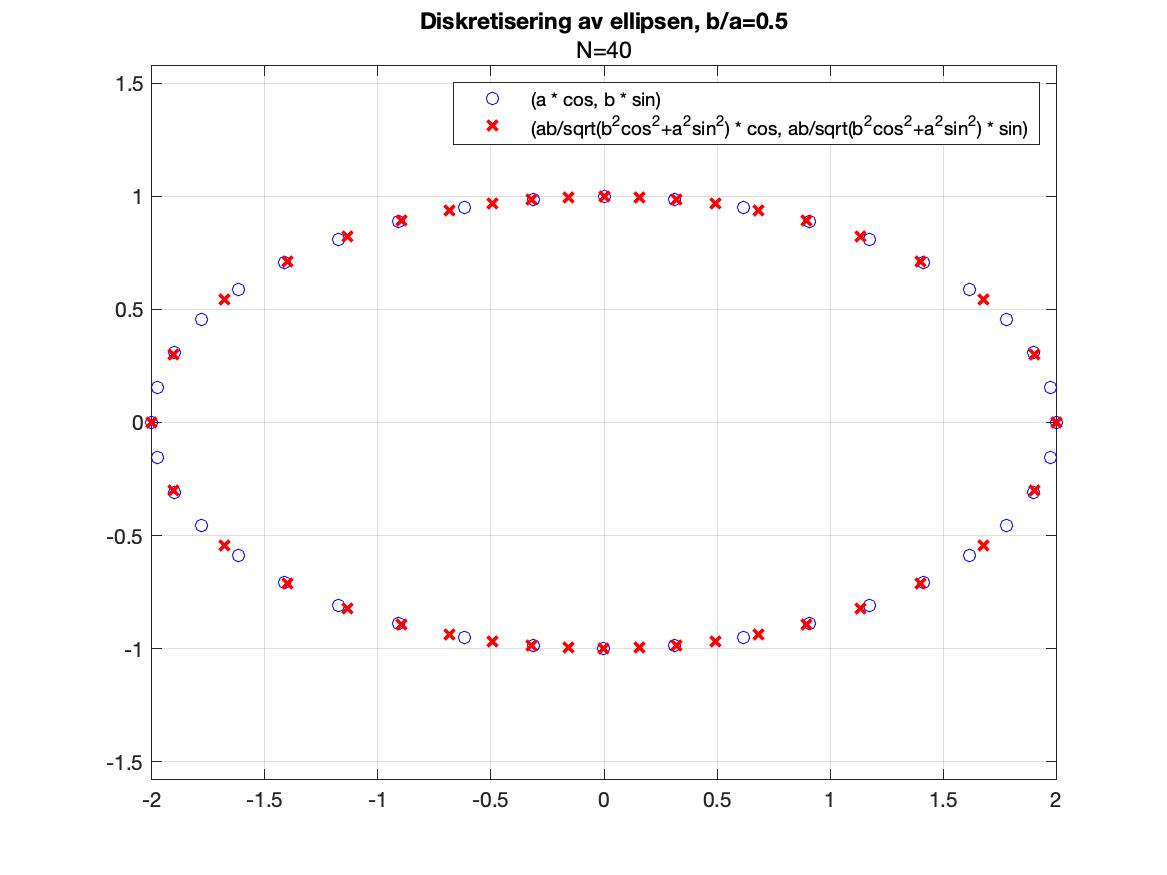
\includegraphics[width=0.8\linewidth]{/Users/ole/Tex/MEK4420/oblig1images/diskretisering_2ellipse.png}
\captionof{figure}{}}


%--------------------kvadrat
\section{Kvadrat - Plott av addert masse og plott av potensialer}

{\noindent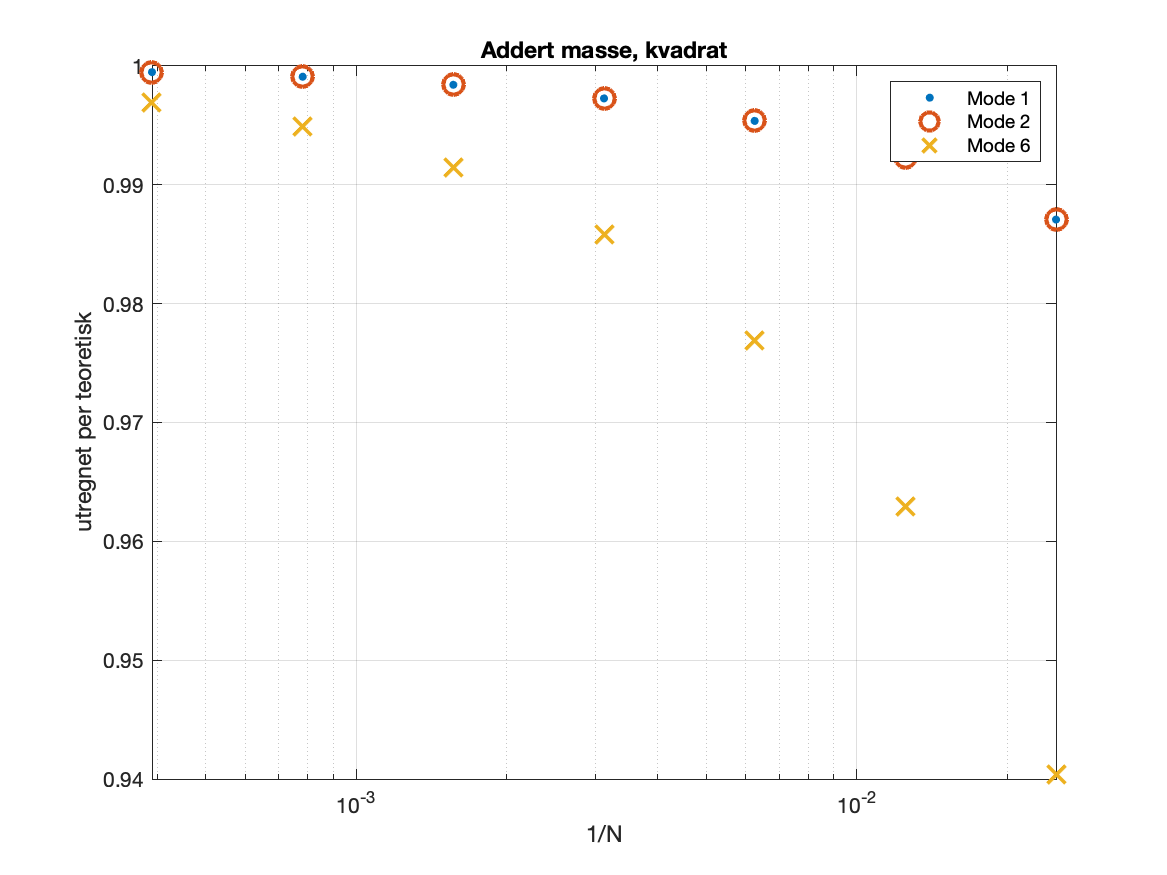
\includegraphics[width=0.8\linewidth]{/Users/ole/Tex/MEK4420/oblig1images/m11_kvadrat.png}
\captionof{figure}{På kvadratet har det blitt brukt ett hakk flere N. Verdier for N = 40,80,160,320,640,1280,2560.}}

{\noindent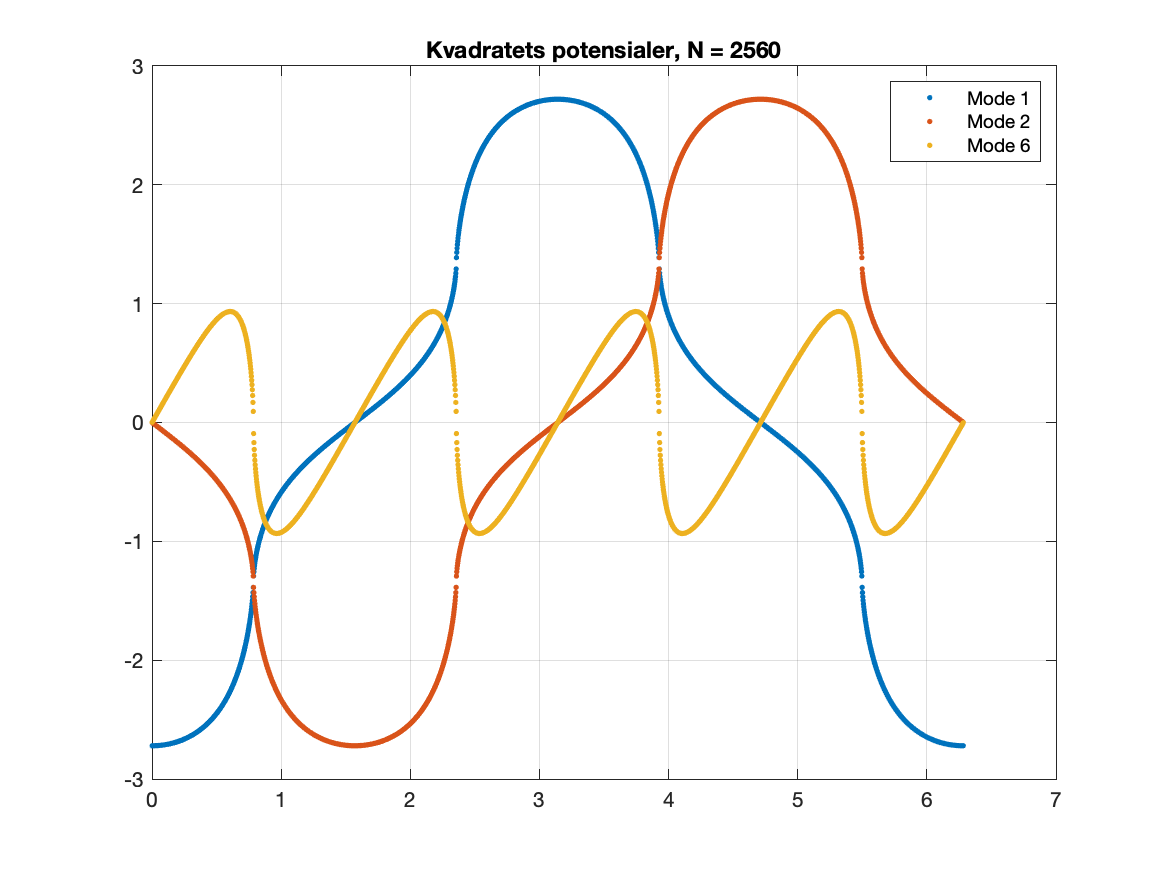
\includegraphics[width=0.8\linewidth]{/Users/ole/Tex/MEK4420/oblig1images/potensialer_kvadrat.png}
\captionof{figure}{Kvadratets potensialer i horisontal og vertikal retning er like. Rotasjonen viser tydelig samme utslag ved hvert hjørne}}

\section{Konklusjoner}
Vi har sett på 3 geometrier: sirkel, ellipse, og kvadrat. Vi har sett at den utregnede adderte massen konvergerer mot den teoretiske, med ulik hastighet, når vi øker N diskretiseringspunkter. Det er fasongen på geometrien som avgjør responsen. 

Videre har vi sett at potensialet på samme vis er avhengig av fasongen på geometrien. En spiss geometri skjærer gjennom mediet, og vil møte mye mindre motstand enn en flat geometri. 


\end{document}

